%%%%%%%%%%%%%%%%%%%%%%%%%%%%%%%%%%%%%%%%%%%%%%%%%%%%%%%%%%%%%%%
%
% Welcome to Overleaf --- just edit your LaTeX on the left,
% and we'll compile it for you on the right. If you give
% someone the link to this page, they can edit at the same
% time. See the help menu above for more info. Enjoy!
%
% Note: you can export the pdf to see the result at full
% resolution.
%
%%%%%%%%%%%%%%%%%%%%%%%%%%%%%%%%%%%%%%%%%%%%%%%%%%%%%%%%%%%%%%%
% Fancy chapter headings
% Author: Stefan Kottwitz 
% Source: http://texblog.net/latex-archive/layout/fancy-chapter-tikz/
\documentclass[12pt,svgnames]{report}
\usepackage{tikz}
\usepackage{verbatim}
\usepackage[margin=1.1in]{geometry}
\usepackage{booktabs}
\usepackage{graphicx}
\usepackage{hyperref}
\usepackage{kpfonts}
 \usepackage{url}
\usepackage[explicit]{titlesec}
\newcommand*\chapterlabel{}
\titleformat{\chapter}
{\gdef\chapterlabel{}
	\normalfont\sffamily\Huge\bfseries\scshape}
{\gdef\chapterlabel{\thechapter\ }}{0pt}
{\begin{tikzpicture}[remember picture,overlay]
	\node[yshift=-1cm] at (current page.north west) %poso paxi tha einai to mple rectangle
	{\begin{tikzpicture}[remember picture, overlay]
		\draw[fill=MidnightBlue] (0,-1) rectangle
		(\paperwidth,2cm);
		\node[anchor=west,xshift=.1\paperwidth,rectangle,
		rounded corners=15pt,inner sep=9pt,
		fill=MidnightBlue]
		{\color{white}\chapterlabel#1};
		\end{tikzpicture}
	};
\end{tikzpicture}
}
\titlespacing*{\chapter}{0pt}{50pt}{-60pt}

\title{Report on Twitter topic detection and analysis}
\author{
Alex Tsilingiris \\
Christina Pardalidou \\
Sotiris Karapostolakis \\
}

\begin{document}
\maketitle
\tableofcontents
\chapter{Introduction}
Text
\chapter{Model description}
\section*{Section}
List me TF sta hashtags? Preprocessing steps?

\chapter{Method implementation details}
\section*{Event detection}
\subsection*{Our approach}
A combination of approaches was used for event detection: Since the dataset was static and filtered based on a query (in our case the word "trump"), terms were considered as living organisms in the given timespan, allowing us to sample a set of tweets as when each term was "most alive", while combining user reputation metrics to select a tweet from a reputable source.
\subsubsection*{Hashtags as terms}
We solely operated on hashtags on this step since they represent an idea or a topic, which in other cases would be difficult, or not as accurate, to define using Natural Language Processing and Machine Learning.
\subsubsection*{The living organism implementation}
We considered a term as most-alive at the point in which it was mostly detected in our dataset. The time window was set to 2 hours. Therefore, we had to query for the mostly found terms (using the Term Frequency statistic) and sort the results in descending order. We then generated the final that contained the original tweets with the most active terms in the dataset that were posted in the given timespan.
\subsubsection*{Selecting a tweet for the pool}
We now have a pool of tweets that might contain information about an event. The approach we followed was to assume that a user with a high amount of followers represents an influential event source  into a social community\cite{cataldi2013personalized}. We sorted (descending) the tweet pool by the number of followers the original poster has and ended up with 1 tweet that was our result for each term.


\chapter{Sample results}
\section*{Event detection}
Some top ranked terms (hashtags), their occurrences and the tweet that qualified as an event by our system will be presented in table \ref{tab:tftags}

\begin{table}[h!]
	\centering

	\begin{tabular}{ccc}
		\toprule
		Term & Frequency\\
		\midrule
		\#parisagreement & 10442\\
		\#covfefe & 7085\\
		\#trumprussia & 4229\\
		\#marchfortruth & 973\\
		\bottomrule
	\end{tabular}
	\caption{Terms and occurrences}
\label{tab:tftags}
\end{table}


The top ranked term, a graph showing its occurrence over time can be seen in the following figure:\\
\\
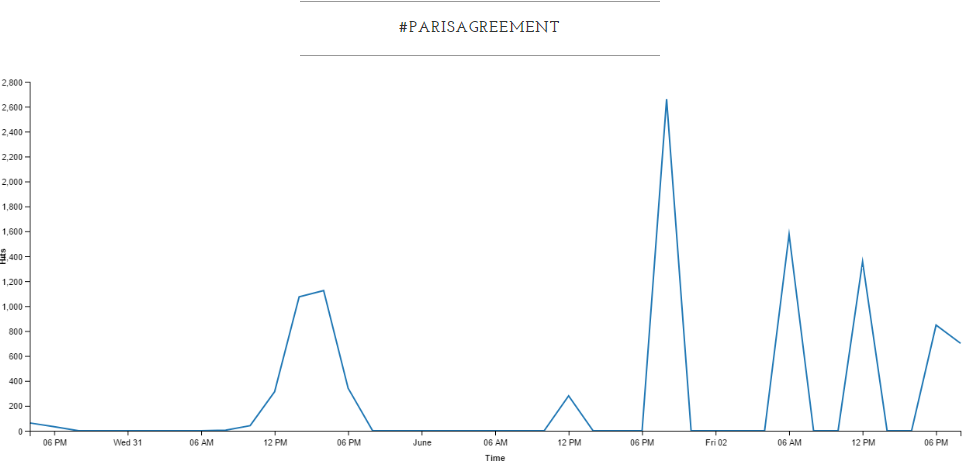
\includegraphics[scale=0.63]{hashparisplot.png}
\\

\newpage
The tweet that our system determined as an event can be seen in the following figure:
\begin{figure}[h]
\centering
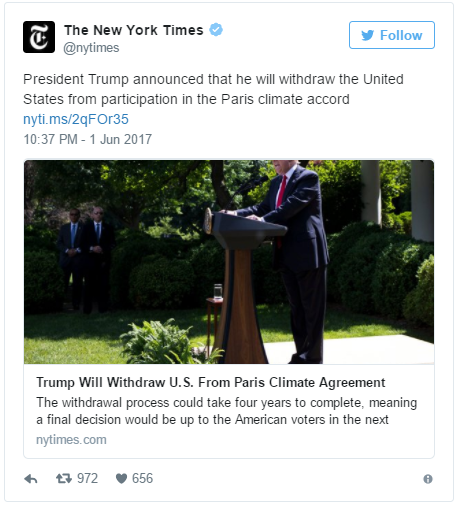
\includegraphics[scale=1]{hashparistweet.png}
\end{figure}
\\
Additional results can be found in the project's website \cite{projectwebsite}.


\chapter{Software implementation details}
\section*{Section}
Test

\bibliographystyle{abbrv}
\bibliography{sigproc}


\end{document}